\documentclass[14pt,a4paper,UTF8,twoside]{article}
% 用 documentclass 来声明文章的类型,一般用 article,可以百度搜搜还有什么可以选
% 12pt 一般是小四的大小,可以查查 pt 是什么单位
% 可以选择 a5、a6 等纸张
% UTF8 是编码格式,要用中文的话, UTF8 是最推荐的编码格式
% twoside 是打印的时候用双面打印,一般用不上

% Formatting Packages ——————————————————————————————————————
\usepackage{multicol} % 多行多列包
\usepackage{multirow}
\usepackage{enumitem} % 数字编号包
\usepackage{indentfirst}
\usepackage[toc]{multitoc} % 多行目录包

% Math & Physics Packages ————————————————————————————
\usepackage{amsmath, amsthm, amsfonts, amssymb} % 基础数学包
\usepackage{setspace}
\usepackage{physics}
\usepackage{cancel}
\usepackage{nicefrac}
\usepackage{unicode-math} % 允许数学公式使用特定字体
\usepackage{mdframed} % 注释包

% Image-related Packages —————————————————————————————
\usepackage{graphicx} % 插入图片要这个包
\usepackage{float} % 浮动体环境,用来调整图片的位置
\usepackage{subcaption} % 子图包
\usepackage{pgfgantt}
\usepackage{graphics, graphicx}
\usepackage{tikz, tikz-qtree}
\usetikzlibrary{arrows.meta, positioning, shapes}
\usetikzlibrary{shapes.geometric}
\tikzstyle{node_style} = [rectangle, rounded corners, draw, align=center, text width=3cm, minimum height=0.65cm]
\tikzstyle{arrow_style} = [thick, ->, >=stealth]

\usepackage{pgfplots}
\pgfplotsset{compat=1.18}
\usepackage{xcolor}
\usepackage{fourier-orns}
\usepackage{lipsum}

% 其余常用包 ————————————————————————————————————————————
\usepackage{booktabs} % 表格库
\usepackage{titlesec} % 标题库
\usepackage{fancyhdr} % 页眉页脚库
\usepackage[sorting=none]{biblatex}
\usepackage{array}

%—————————————页面基础设置———————————————%

\usepackage{geometry}
\geometry{left=10mm, right=10mm, top=20mm, bottom=20mm}
% 这个命令用来设置纸张上下左右的间距,可以自己调调试试

% 字体设置 ————————————————————————————————————————————————
\usepackage{fontspec} % 允许设置字体
\usepackage[utf8]{inputenc}
\usepackage{ctex}

% 代码块包 ————————————————————————————————————————————————
\usepackage{listings}

% ————————————————————————————————————————————————————————

\title{LateX 入门}

\begin{document}

\maketitle % 用来显示上面写的 \title{LateX 入门}

\section{LateX 是以环境为主的}

在 VSCode 中,Ctrl + Alt + B 是编译成 PDF 的快捷键.

\subsection{居中显示}

\begin{center}
    使用 center 来创建居中环境,注意,反斜杠符号是特殊符号,
    在 LateX 里是告诉编译器:我要开始一条命令了,所以直接输入反斜杠是不能显示的,
    要转义,转义的方法是输入三个斜杠 \\\
\end{center}

\textbf{文字加粗},\textit{文字斜体},\underline{文字下划线},代码用等宽字体:\texttt{This is some code}

% 在 figure 环境后添加 [H],这个是固定的,用来让这个图片进入浮动体环境,如果不添加这个 [H],图片可能不会按照你想要的位置排,所以每次插入图片都要加上 [H]

\begin{figure} [H]
    \centering % 图片居中的命令
    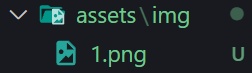
\includegraphics[width=0.5\textwidth]{../assets/img/1.png} % 可以自己调一下 width 的值试试
    \caption{示例图片标题}
    \label{fig:my_label} % 设置标签,以便后续引用
\end{figure}

要注意一下怎么对路径进行引用。像这个项目里,结构如下:

\begin{lstlisting}
    project/
    │
    ├── assets/
    │   ├── examples/
    │   └── img/
    │       └── 1.png
    │
    ├── report/
    │   ├── begin.aux
    │   ├── begin.bcf
    │   ├── begin.log
    │   ├── begin.pdf
    │   ├── begin.run.xml
    │   ├── begin.synctex.gz
    │   └── begin.tex
    │
    └── src/
        └── question1.py    
\end{lstlisting}

tex 文件是你编辑的文件,要找到你的图片,向上返回一层后,到 report,再向上返回一层,到 project 的根目录,然后进入 assets,再进入 img,然后找到了 1.png,所以要用 ../assets/img/1.png

这里是引用图片的例子:如图 \ref{fig:my_label} 所示。 % 这里对图片进行引用

\subsection{子标题}

\subsubsection{子子标题}

\end{document}
